\documentclass[tikz,11pt,a4paper,booktabs,notitlepage]{report}
\usepackage[utf8]{inputenc}
\usepackage[T1]{fontenc}
%\usepackage{amsmath}
%\usepackage{amsfonts}
%\usepackage{amssymb}
\usepackage{fullpage}
\usepackage[margin=1cm]{geometry}
%\usepackage{fancyhdr}
%\usepackage{fancybox}
\usepackage[table]{xcolor}
\usepackage{graphicx}
\usepackage{multicol}
\usepackage{booktabs}
\usepackage{todonotes}
\usepackage{./karnaugh-map}
\usepackage{tikz}
\usetikzlibrary{arrows, shapes.gates.logic.US, calc}

\usepackage[utf]{arabxetex}

%define arabtex
%\newcommand{\aRL}{\RL} 
% use arab xe tex, need defining RL
\newcommand{\aRL}{\textarab[utf]} 
\newfontfamily\arabicfont[Script=Arabic]{Amiri}
\author{Taha Zerrouki}
\setlength{\headheight}{2pt}
\begin{document}
\textbf{Université de Bouira}\hfill \textbf{Faculté de sciences}\\[8pt]
\textbf{\LARGE{Test n °3}} \hfill Module: \textbf{Structure Machine 1}\\[5pt]
\large{Nom \& Prénom}\dotfill \hfill \large{Groupe:}\dotfill\\
\rule{\textwidth}{1pt}

\paragraph{Exercice 1}

%\begin{minipage}{7cm}

%\end{minipage}\hfill
%\begin{minipage}{11cm}
%
%\end{minipage}
%\begin{minipage}{8cm}
%
%\end{minipage}\hfill
%\begin{minipage}{10cm}
%
%\end{minipage}
%\begin{minipage}{11cm}
%\end{minipage}
Etudier la fonction suivante

F = R([6, 7])
%%\begin{table}
        \begin{tabular}{|c|c|c|c|c||c|}
    \toprule
         & A & B & C & D & F\\ \midrule0 & 0 & 0 & 0 & 0 & 0\\1 & 0 & 0 & 0 & 1 & 0\\2 & 0 & 0 & 1 & 0 & 0\\3 & 0 & 0 & 1 & 1 & 0\\\midrule4 & 0 & 1 & 0 & 0 & 0\\5 & 0 & 1 & 0 & 1 & 0\\6 & 0 & 1 & 1 & 0 & 1\\7 & 0 & 1 & 1 & 1 & 1\\\midrule8 & 1 & 0 & 0 & 0 & 0\\9 & 1 & 0 & 0 & 1 & 0\\10 & 1 & 0 & 1 & 0 & 0\\11 & 1 & 0 & 1 & 1 & 0\\\midrule12 & 1 & 1 & 0 & 0 & 0\\13 & 1 & 1 & 0 & 1 & 0\\14 & 1 & 1 & 1 & 0 & 0\\15 & 1 & 1 & 1 & 1 & 0\\\bottomrule
        \end{tabular}
        %%\end{table}
        
Sum of products 
 f(a,b,c,d) = $\bar a.b.c.\bar d + \bar a.b.c.d$

Product of sums 
 f(a,b,c,d) = $a.b.c.d.a.b.c.\bar d.a.b.\bar c.d.a.b.\bar c.\bar d.a.\bar b.c.d.a.\bar b.c.\bar d.\bar a.b.c.d.\bar a.b.c.\bar d.\bar a.b.\bar c.d.\bar a.b.\bar c.\bar d.\bar a.\bar b.c.d.\bar a.\bar b.c.\bar d.\bar a.\bar b.\bar c.d.\bar a.\bar b.\bar c.\bar d$

Karnough map\todo{fix map}
\begin{karnaugh-map}[4][4][1][cd][ab]
          \minterms{6, 7}
          \maxterms{0, 1, 2, 3, 4, 5, 8, 9, 10, 11, 12, 13, 14, 15}
        %\autoterms[0]
          %\implicant{5}{15}
          %\implicantedge{8}{8}{10}{10}
          %\implicantedge{8}{8}{10}{10}[8,10]
        \end{karnaugh-map}

Simplified Sum of products: $\bar a.b.c$

Simplified Product of sums: $b.c.\bar a$
\paragraph{Logigramme} de la fonction\\
        %%\missingfigure[figwidth=6cm]{Logigramme}

 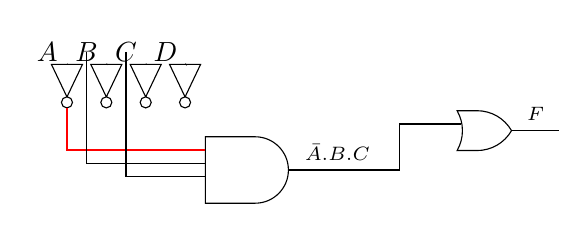
\begin{tikzpicture}

\node (x) at (0, 1*1.5) {$A$};
            \node (y) at (0.5, 1*1.5) {$B$};
            \node (z) at (1, 1*1.5) {$C$};
            \node (w) at (1.5, 1*1.5) {$D$};
            \node[not gate US, draw, rotate=270] at ($(x) + (0.25, -0.3)$) (notx) {};
            \draw (x) -- (notx.input); 
            \node[not gate US, draw, rotate=270] at ($(y) + (0.25, -0.3)$) (noty) {};
            \draw (y) -- (noty.input); 
            \node[not gate US, draw, rotate=270] at ($(z) + (0.25, -0.3)$) (notz) {};
            \draw (z) -- (notz.input);
            \node[not gate US, draw, rotate=270] at ($(w) + (0.25, -0.3)$) (notw) {};
            \draw (w) -- (notw.input);
                
           
            \node[and gate US, draw, rotate=0, logic gate inputs=nnnn] at (2.5, 0*1.5) (xandy0) {};
            \draw (xandy0.output) -- node[above]{\scriptsize $\bar A.B.C$} ($(xandy0) + (1.8, 0)$);
            
            %% X'

            \draw  [line width=0.25mm,   red] (notx.output) -- ([xshift=0cm]notx.output) |- (xandy0.input 1);
              
            %% Y
            \draw (y) -| ($(y) + (0, 0)$) |- (xandy0.input 2);
        
            %%Z
            \draw (z) -| ($(z) + (0, 0)$) |- (xandy0.input 3);
        \node[or gate US, draw, rotate=0, logic gate inputs=nn] at (5.5, 1*0.5) (xory) {};


                    \draw (xory.output) -- node[above]{\scriptsize$F$} ($(xory) + (1, 0)$);

\draw (xandy0.output) -- ([xshift=1.40cm]xandy0.output) |- (xory.input 1);

 \end{tikzpicture}


\pagebreak\section{Questions}



\end{document}